\documentclass{article}
\usepackage{graphicx}
\graphicspath{ {images/} }
\usepackage{float}

% alternative font if you prefer
% \usepackage{times}

% for alternative page numbering use the following package
% and see documentation for commands
\usepackage{fancyheadings}
\usepackage{hyperref}


% other potentially useful packages
\usepackage{amssymb,amsmath}
%\usepackage{url}
%\usepackage{fancyvrb}
%\usepackage[final]{pdfpages}
\setlength{\parindent}{0pt}
\setlength{\parskip}{11pt plus 2pt}

\begin{document}

%%%%%%%%%%%%%%%%%%%%%%%%%%%%%%%%%%%%%%%%%%%%%%%%%%%%%%%%%%%%%%%%%%%
\title{Report: Generative Processes of Static and Dynamic LDA Models}
\author{Arijus Pleska}
\maketitle

%%%%%%%%%%%%%%%%%%%%%%%%%%%%%%%%%%%%%%%%%%%%%%%%%%%%%%%%%%%%%%%%%%%

% - Comparing the static and dynamics models.
% - Questions 
\par During this week I have familiarised with the generative processes of static and dynamic LDA models. In this report I will present the results by plotting the generated corpora, address the initialisation of the parameters $\alpha$ and $\beta$, and raise questions for the next meeting.

% Generative process
\par I have managed to generate documents using both static and dynamic variations. The static approach in generating corpus is given in Figure 1, and the dynamic approach is given in Figure 2.

\begin{figure}[H]
  \centering
  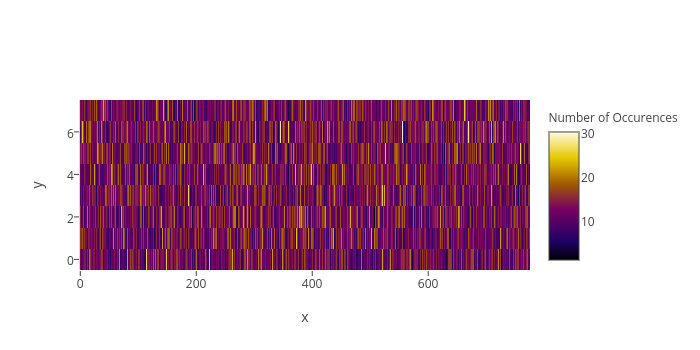
\includegraphics[width=\textwidth]{static}
  \caption{The distribution of a word in a corpus produced by the static generative process.}
  \label{fig:static}
\end{figure}

\begin{figure}[H]
  \centering
  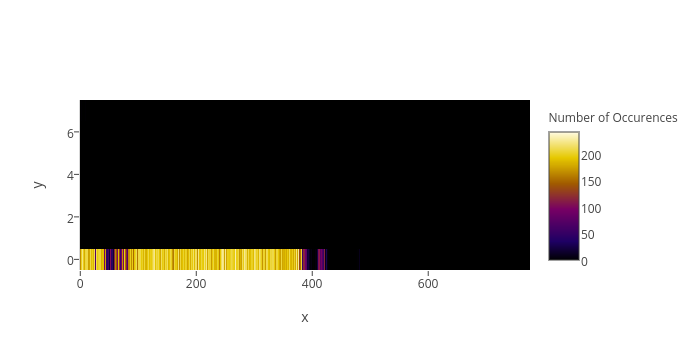
\includegraphics[width=\textwidth]{dynamic}
  \caption{The distribution of a word in a corpus produced by the dynamic generative process.}
  \label{fig:dynamic}
\end{figure}

In Figure 1 we can see that the word is present throughout the corpus, whereas Figure 2 displays a smoother distribution of the word. That is, the dynamic generative process induces a structure of the word's existence in the corpus. Also, note that both corpus contain the same number of documents and the number of words in a document is drawn from the Poisson distribution on the same mean $\xi = 200$.

The implementation of the generative processes follows directly from the original LDA paper \cite{Blei:2003:LDA:944919.944937} and the paper on dynamic topic models \cite{Blei:2006:DTM:1143844.1143859}. The Python Notebook containing the implementation of the processes can be found on the following link: \url{https://github.com/perdaug/mlinb/blob/master/notebooks/generating_corpus.ipynb}. Note that the initial values of the parameter $\alpha$ are positive and random, whereas the initial values of the parameter $\beta$ are equal and normalised for each topic. This formulation of $\beta$ suggests that each word has an equal probability of getting drawn in the first document generation of the dynamic model and throughout all generated documents of the static model. Also, note that every generated document in the dynamic model is unique with respect to other documents. In other words, each dynamic time-slice contains one document. 

During the upcoming meeting I would like to address the following questions:
\begin{enumerate}
\item Should we use the variational inference for the implementation of the dynamic topic model? If not, would Gibbs sampling scale with the future datasets?
\item Why Dirichlet distribution is amenable in the dynamic topic modelling? (This is claimed in the last paragraph of the first page of the dynamic topic modelling paper \cite{Blei:2006:DTM:1143844.1143859})
\item For the dynamic model implementation, should we update $\alpha_{t-1}$ (as discussed in Subsection 5.3 of the original LDA paper \cite{Blei:2003:LDA:944919.944937}) before drawing $\alpha_t$? 
\end{enumerate}

\bibliographystyle{unsrt}
\bibliography{report_generative-process}

\end{document}
